\documentclass{article}

\usepackage{amsmath}
\usepackage{amsfonts} % For math fonts.
\usepackage{amssymb} % For other math symbols not covered by amsmath.
\usepackage[pdftex]{graphicx} % For pictures, use \includegraphics[scale=decimal]{pic.png}; must be a .png file type.
\usepackage{multicol}
\usepackage{textcomp}
\usepackage[colorlinks = true, urlcolor = blue]{hyperref}
\usepackage{enumitem}
\usepackage{graphbox} 
\usepackage{subfig}
\usepackage{multicol}
\usepackage{nopageno}
\usepackage{bm}


\usepackage{tikz}
\usetikzlibrary{positioning, calc}
\usetikzlibrary{shapes.geometric,angles,quotes}
\usepackage{tikz-3dplot}


%page formatting
\usepackage{fullpage}
\setlength{\parindent}{0pt}


\newcommand{\tab}{\hspace*{0.25in}}
\newcommand{\csq}[1]{\reflectbox{''}#1''}  %This produces CS style quotes.
\newcommand{\csqt}[1]{\text{\reflectbox{''}#1''}}  %This produces CS style quotes as text.


\usepackage{listings}
\lstset
{ %Formatting for code in appendix
    language=Python,
    basicstyle=\footnotesize,
    numbers=left,
    stepnumber=1,
    showstringspaces=false,
    tabsize=2,
    breaklines=true,
    breakatwhitespace=false,
}


\begin{document}



%split_point

%\end{document}
Lone Star \hfill Midterm quiz\\
section 4\\
\begin{enumerate}
\item (1.2) Write a program that asks the user for \\
		\begin{minipage}{0.5\textwidth}
		\vspace*{-0.5em}
			\begin{enumerate}  \setlength\itemsep{-0.3em}
				\item their first name and
				\item their age.  
			\end{enumerate} \vspace*{-1ex}
		and then outputs a greeting.
		\end{minipage}
		%\
		\begin{minipage}{0.5\textwidth}
			\centering
			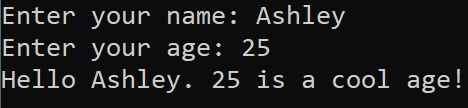
\includegraphics[scale=0.95]{./imgs/outputGreetingWithAge.png}\\
			Your output should be similar to this.
		\end{minipage}




\item (1.3) 
		Write code to swap the values of $x$ and $y$ using a temporary variable and without using
		the built-in function swap().\\		
		\begin{tabular}{|ll}
			\\			
			x = 3\\
			y = 7\\[5pt]
			\#Your code here. \\[5pt]
			& \\ & \\ & \\ & \\ & \\ & \\ & \\ & \\ & \\ & \\ 
		\end{tabular}


%end_of_questions

\item (3.2)  
		Write a program that prompts the user to enter three integers and displays the integers 
		in increasing order (smallest to largest).  You may not use the built-in functions 
		\textit{max}(), \textit{min}(), \textit{sort}() or \textit{sorted}().


\item (3.3)  
		The table below shows the maximum health of characters based on race and class for a new 
		video game I am creating.  Write a program that asks the user for the race and the class of 
		their character, and then sets the \textit{health\_points}	variable according to the table 
		below.
		\begin{flushright}
		\begin{tabular}{c|cc}
			& \multicolumn{2}{c}{Race}\\
			Class & Elf & Ogre \\ \hline
			Warrior & 150 & 200\\
			Bard & 75 & 100\\
			Wizard & 25 & 50 \\
		\end{tabular}
		\end{flushright}
		
		\vspace*{-6em}
		\textit{health\_points} = -1\\
		\#Your code here.
		\vspace*{3em}





\item (4.1)  
		Write a program that asks the user for a word and then, \underline{using a loop}, 
		prints every other letter of the word starting with the second letter.

		Examples:
		\begin{itemize}
			\item if user\_word = \csq{counterattack}, the result should be \csq{oneatc}
			\item if user\_word = \csq{banana sunday}, the result should be \csq{aaasna}
		\end{itemize}


\end{enumerate}
\pagebreak
Dot Matrix \hfill Midterm quiz\\
section 5\\
\begin{enumerate}
\item (1.2) Write a program that asks the user for \\
		\begin{minipage}{0.5\textwidth}
		\vspace*{-0.5em}
			\begin{enumerate}  \setlength\itemsep{-0.3em}
				\item their first name and
				\item their age.  
			\end{enumerate} \vspace*{-1ex}
		and then outputs a greeting.
		\end{minipage}
		%\
		\begin{minipage}{0.5\textwidth}
			\centering
			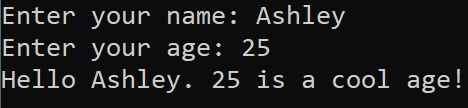
\includegraphics[scale=0.95]{./imgs/outputGreetingWithAge.png}\\
			Your output should be similar to this.
		\end{minipage}




\item (1.3) 
		Write code to swap the values of $x$ and $y$ using a temporary variable and without using
		the built-in function swap().\\		
		\begin{tabular}{|ll}
			\\			
			x = 3\\
			y = 7\\[5pt]
			\#Your code here. \\[5pt]
			& \\ & \\ & \\ & \\ & \\ & \\ & \\ & \\ & \\ & \\ 
		\end{tabular}


%end_of_questions

\item (3.2)  
		In Harry Potter, the currency consists of knuts, sickle, and galleon.  There are 29 knuts in 
		one sickle and 17 sickles in one galleon.  Write a program that will convert some amount of 
		knuts into the fewest amount of coins possible.  Only print non-zero values, meaning don't 
		print something similar to ``0 sickles.''  For example,
		\begin{itemize}
			\item Given 32 knuts, output 1 sickle 3 knuts
			\item Given 544 knuts, output 1 galleon 4 sickles 18 knuts
			\item Given 993 knuts, output 2 galleons 7 knuts. 
				Do \textbf{not} output 2 galleons 0 sickle 7 knuts.
		\end{itemize}




\item (3.3)  
		The table below show what your resting heart rate should be based on age and athleticism.  
		Write a program that asks the user their age and desired athleticism goal, and then outputs 
		what their resting heart rate should be.

		\begin{minipage}{.45\textwidth}
			\begin{tabular}{c|cc}
				& \multicolumn{2}{c}{Athleticism}\\
				Age & Above Average & Below Average \\ \hline
				20 -- 39 & 47 -- 72 & 73 -- 93\\
				40 -- 59 & 46 -- 71 & 72 -- 94\\
				60 -- 79 & 45 -- 70 & 71 -- 97 \\
			\end{tabular}
		\end{minipage}
		\begin{minipage}{.45\textwidth}
			\vspace*{1em}
			Your end output should look similar to this
			\fbox{\parbox{\textwidth}{ Enter your age: 45\\
			Enter your athleticism goal: Below Average\\
			Your resting heart rate should be between 72--94.}}
		\end{minipage}





\item (4.1)  
		%https://edabit.com/challenge/aqDGJxTYCx7XWyPKc
		Write a program that asks the user for an integer.  Calculate (and then print) the 
		sum of all square numbers up to and including the user's number.

		For example, 
		\begin{itemize}
			\item if user\_number = 3, the result should be 14 since $1^2 + 2^2 + 3^2 = 14$.
			\item if user\_number = 8, the result should be $1^2+2^2+3^2+4^2+5^2+6^2+7^2+8^2=204$.
		\end{itemize}

%end_of_questions

\end{enumerate}
\pagebreak
Dark Helmet \hfill Midterm quiz\\
section 4\\
\begin{enumerate}
\item (1.2) 
		Write a program that asks the user for \\
		\begin{minipage}{0.5\textwidth}
		\vspace*{-0.5em}
			\begin{enumerate}  \setlength\itemsep{-0.3em}
				\item their first name and
				\item their last name.  
			\end{enumerate} \vspace*{-1ex}
		and then outputs a farewell.
		\end{minipage}
		%\
		\begin{minipage}{0.5\textwidth}
			\centering
			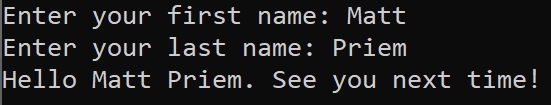
\includegraphics[scale=0.9]{./imgs/outputFarewell.png}\\
			Your output should be similar to this.
		\end{minipage}



\item (1.3) 
		Write code to swap the values of $x$ and $y$ using a temporary variable and without using
		the built-in function swap().\\		
		\begin{tabular}{|ll}
			\\			
			x = 3\\
			y = 7\\[5pt]
			\#Your code here. \\[5pt]
			& \\ & \\ & \\ & \\ & \\ & \\ & \\ & \\ & \\ & \\ 
		\end{tabular}


%end_of_questions

\item (3.2)  
		%https://edabit.com/challenge/ancAxGEF9MsLWXDqe
		Write a program that asks the user for three side lengths of a triangle, and prints 
		the type of triangle.  The types of triangles are 
		\begin{itemize}
			\item No sides equal: \csq{scalene}
			\item Two sides equal: \csq{isosceles}
			\item All sides equal: \csq{equilateral}	
		\end{itemize}
		For example:

		\hfill 
		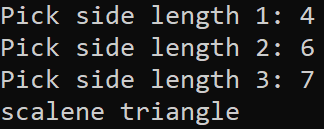
\includegraphics[height = 0.7in]{./imgs/typeOfTriangle1.PNG} \hfill 
		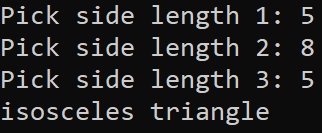
\includegraphics[height = 0.7in]{./imgs/typeOfTriangle2.PNG} \hfill  
		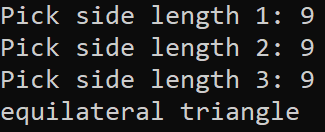
\includegraphics[height = 0.7in]{./imgs/typeOfTriangle3.PNG} \hfill \ 




%end_of_questions








\item (3.3)  
		The table below shows what time different age groups (by grade) can swim at the pool.  There 
		are two time options, morning and afternoon.  Write a program that asks the user their grade 
		and whether they'd like to go in the morning or afternoon, and outputs the time the pool is 
		available for them.

		\begin{minipage}{.45\textwidth}
		\begin{tabular}{c|cc}
						& \multicolumn{2}{c}{Pool times}\\
			Grade 		& Morning 	& Afternoon \\ \hline
			k, 1 -- 3 	& 9 AM 		& 1 PM\\
			4 -- 8 		& 10 AM 	& 2 PM\\
			9 -- 12 	& 11 AM 	& 3 PM \\
		\end{tabular}
		\end{minipage}
		%
		\begin{minipage}{.45\textwidth}
			\ \\
			Your end output should look similar to this
			%(if you were to actually run the code).

			\fbox{\parbox{\textwidth}{ Enter your grade: 5\\
			Enter Morning OR Afternoon: Morning\\
			The pool is open at 10 AM.}}
		\end{minipage}



%end_of_questions








\item (4.1)  
		Using a loop, write a program that prints every even number 
		between 37 and 1050 (inclusively).


\end{enumerate}
\pagebreak
President Skroob \hfill Midterm quiz\\
section 1\\
\begin{enumerate}
\item (1.2) 
		Write a program that asks the user for \\
		\begin{minipage}{0.5\textwidth}
		\vspace*{-0.5em}
			\begin{enumerate}  \setlength\itemsep{-0.3em}
				\item their first name and
				\item their last name.  
			\end{enumerate} \vspace*{-1ex}
		and then outputs a greeting.
		\end{minipage}
		%\
		\begin{minipage}{0.5\textwidth}
			\centering
			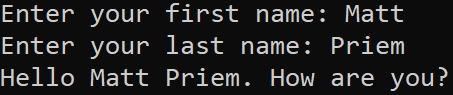
\includegraphics[scale=0.9]{./imgs/outputGreeting.png}\\
			Your output should be similar to this.
		\end{minipage}

%end_of_questions

\item (1.3) 
		Write code to swap the values of $x$ and $y$ using a temporary variable and without using
		the built-in function swap().\\		
		\begin{tabular}{|ll}
			\\			
			x = 3\\
			y = 7\\[5pt]
			\#Your code here. \\[5pt]
			& \\ & \\ & \\ & \\ & \\ & \\ & \\ & \\ & \\ & \\ 
		\end{tabular}


%end_of_questions

\item (3.2)  
		Primary U.S. interstate highways are numbered 1-99.  Odd numbers (like 5 or 95) go north/
		south, and evens (like 10 or 82) go east/west.  Auxiliary highways are numbered 100-999, and 
		service the primary highway indicated by the rightmost two digits.  Thus, I-405 services 
		I-5, and I-290 services I-90.
		
		Note: 200 is not a valid auxiliary highway because 00 is not a valid primary highway 
		number.\\
		
		Let the user pick a highway number.  Given a valid highway number, indicate whether it runs 
		north/south or east/west.  If it is an invalid highway number, indicate that it is an 
		invalid highway number. \\
		For example,
		
		\hfill
		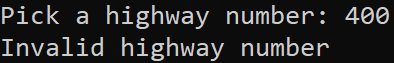
\includegraphics[width = 2in]{./imgs/highwayValidator1.PNG} \hfill
		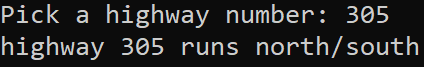
\includegraphics[width = 2in]{./imgs/highwayValidator2.PNG} \hfill \ 

		\hfill 
		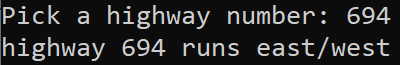
\includegraphics[width = 2in]{./imgs/highwayValidator3.PNG} \hfill 
		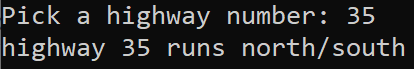
\includegraphics[width = 2in]{./imgs/highwayValidator4.PNG} \hfill \ 



\item (3.3)  
		The table below show what your resting heart rate should be based on age and athleticism.  
		Write a program that asks the user their age and desired athleticism goal, and then outputs 
		what their resting heart rate should be.

		\begin{minipage}{.45\textwidth}
			\begin{tabular}{c|cc}
				& \multicolumn{2}{c}{Athleticism}\\
				Age & Above Average & Below Average \\ \hline
				20 -- 39 & 47 -- 72 & 73 -- 93\\
				40 -- 59 & 46 -- 71 & 72 -- 94\\
				60 -- 79 & 45 -- 70 & 71 -- 97 \\
			\end{tabular}
		\end{minipage}
		\begin{minipage}{.45\textwidth}
			\vspace*{1em}
			Your end output should look similar to this
			\fbox{\parbox{\textwidth}{ Enter your age: 45\\
			Enter your athleticism goal: Below Average\\
			Your resting heart rate should be between 72--94.}}
		\end{minipage}





\item (4.1)  
		%https://edabit.com/challenge/6Pf5GGG6HnzbB95gf
		Write code that asks the user for an integer and then prints each number that is a 
		factor of the input.
	
		For example, \\ \ \hfill
		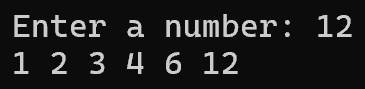
\includegraphics[height = .35in]{./imgs/factors1.PNG} \hfill  
		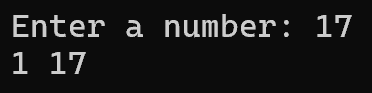
\includegraphics[height = .35in]{./imgs/factors2.PNG} \hfill  
		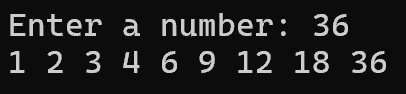
\includegraphics[height = .35in]{./imgs/factors3.PNG} \hfill \


\end{enumerate}
\pagebreak
Hal 9000 \hfill Midterm quiz\\
section 0\\
\begin{enumerate}
\item (1.2) Write a program that asks the user for \\
		\begin{minipage}{0.5\textwidth}	
		\vspace*{-0.5em}
			\begin{enumerate}  \setlength\itemsep{-0.3em}
				\item the year,
				\item the month, and
				\item the day	
			\end{enumerate} \vspace*{-1ex}
		and then outputs the date.
		\end{minipage}
		%\
		\begin{minipage}{0.5\textwidth}
			\centering
			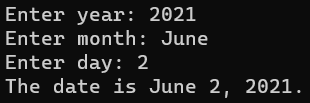
\includegraphics[scale=0.75]{./imgs/dateOutput.png}\\
			Your output should be similar to this.
		\end{minipage}

	

\item (1.3) 
		Write code to swap the values of $x$ and $y$ using a temporary variable and without using
		the built-in function swap().\\		
		\begin{tabular}{|ll}
			\\			
			x = 3\\
			y = 7\\[5pt]
			\#Your code here. \\[5pt]
			& \\ & \\ & \\ & \\ & \\ & \\ & \\ & \\ & \\ & \\ 
		\end{tabular}


%end_of_questions

\item (3.2)  
		%https://edabit.com/challenge/b8wRDMWgMZTN2nmfx
		Ask the user for three integers.  Determine (and output) how many copies of the same number 
		the user entered.\\
		For example, \\ \ \hfill
		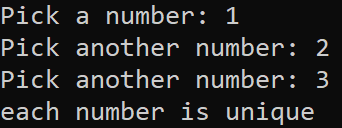
\includegraphics[height = 0.6in]{./imgs/uniqueIntCount1.PNG} \hfill
		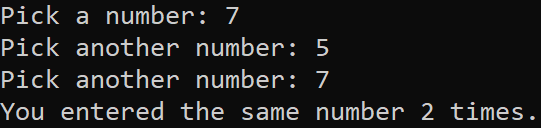
\includegraphics[height = 0.6in]{./imgs/uniqueIntCount2.PNG} \hfill \ 

	
\item (3.3)  
		The table below shows the maximum health of characters based on race and class for a new 
		video game I am creating.  Write a program that asks the user for the race and the class of 
		their character, and then sets the \textit{health\_points}	variable according to the table 
		below.
		\begin{flushright}
		\begin{tabular}{c|cc}
			& \multicolumn{2}{c}{Race}\\
			Class & Elf & Ogre \\ \hline
			Warrior & 150 & 200\\
			Bard & 75 & 100\\
			Wizard & 25 & 50 \\
		\end{tabular}
		\end{flushright}
		
		\vspace*{-6em}
		\textit{health\_points} = -1\\
		\#Your code here.
		\vspace*{3em}





\item (4.1)  
		%https://edabit.com/challenge/6Pf5GGG6HnzbB95gf
		Write code that asks the user for an integer and then prints each number that is a 
		factor of the input.
	
		For example, \\ \ \hfill
		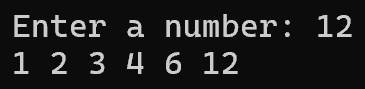
\includegraphics[height = .35in]{./imgs/factors1.PNG} \hfill  
		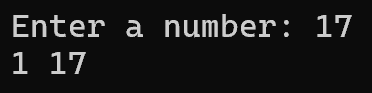
\includegraphics[height = .35in]{./imgs/factors2.PNG} \hfill  
		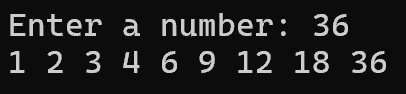
\includegraphics[height = .35in]{./imgs/factors3.PNG} \hfill \


\end{enumerate}
\pagebreak
\end{document}